\chapter{Architektura}

\section{Rozdělení do balíčků}

Aplikaci lze rozdělit do několika balíčků, i když toto rozdělení není tak patrné jako například u Javy. Jako vzor pro celkovou architekturu bylo zvoleno MVC (model-view-controller), kde je oddělená prezentační část od výkonné a obsahové. Nicméně to vyžadovalo pár kompromisů protože JavaScript není primárně objektový jazyk.

Celá aplikace využívá ke svému běhu knihovnu PrototypeJS\cite{prototypejs}, díky které lze snadno definovat objekty a omezeně i dědičnost mezi nimi. V prezentační části se navíc využívá knihovna Script.aculo.us\cite{scriptaculous}, která je postavena na dříve zmíněném PrototypeJS a která umožňuje snadnější vytváření efektů a různých animací.

Diagram \ref{fig:class-model} znázorňuje rozdělení aplikace do balíčků.

\begin{figure}[h]
\begin{center}
	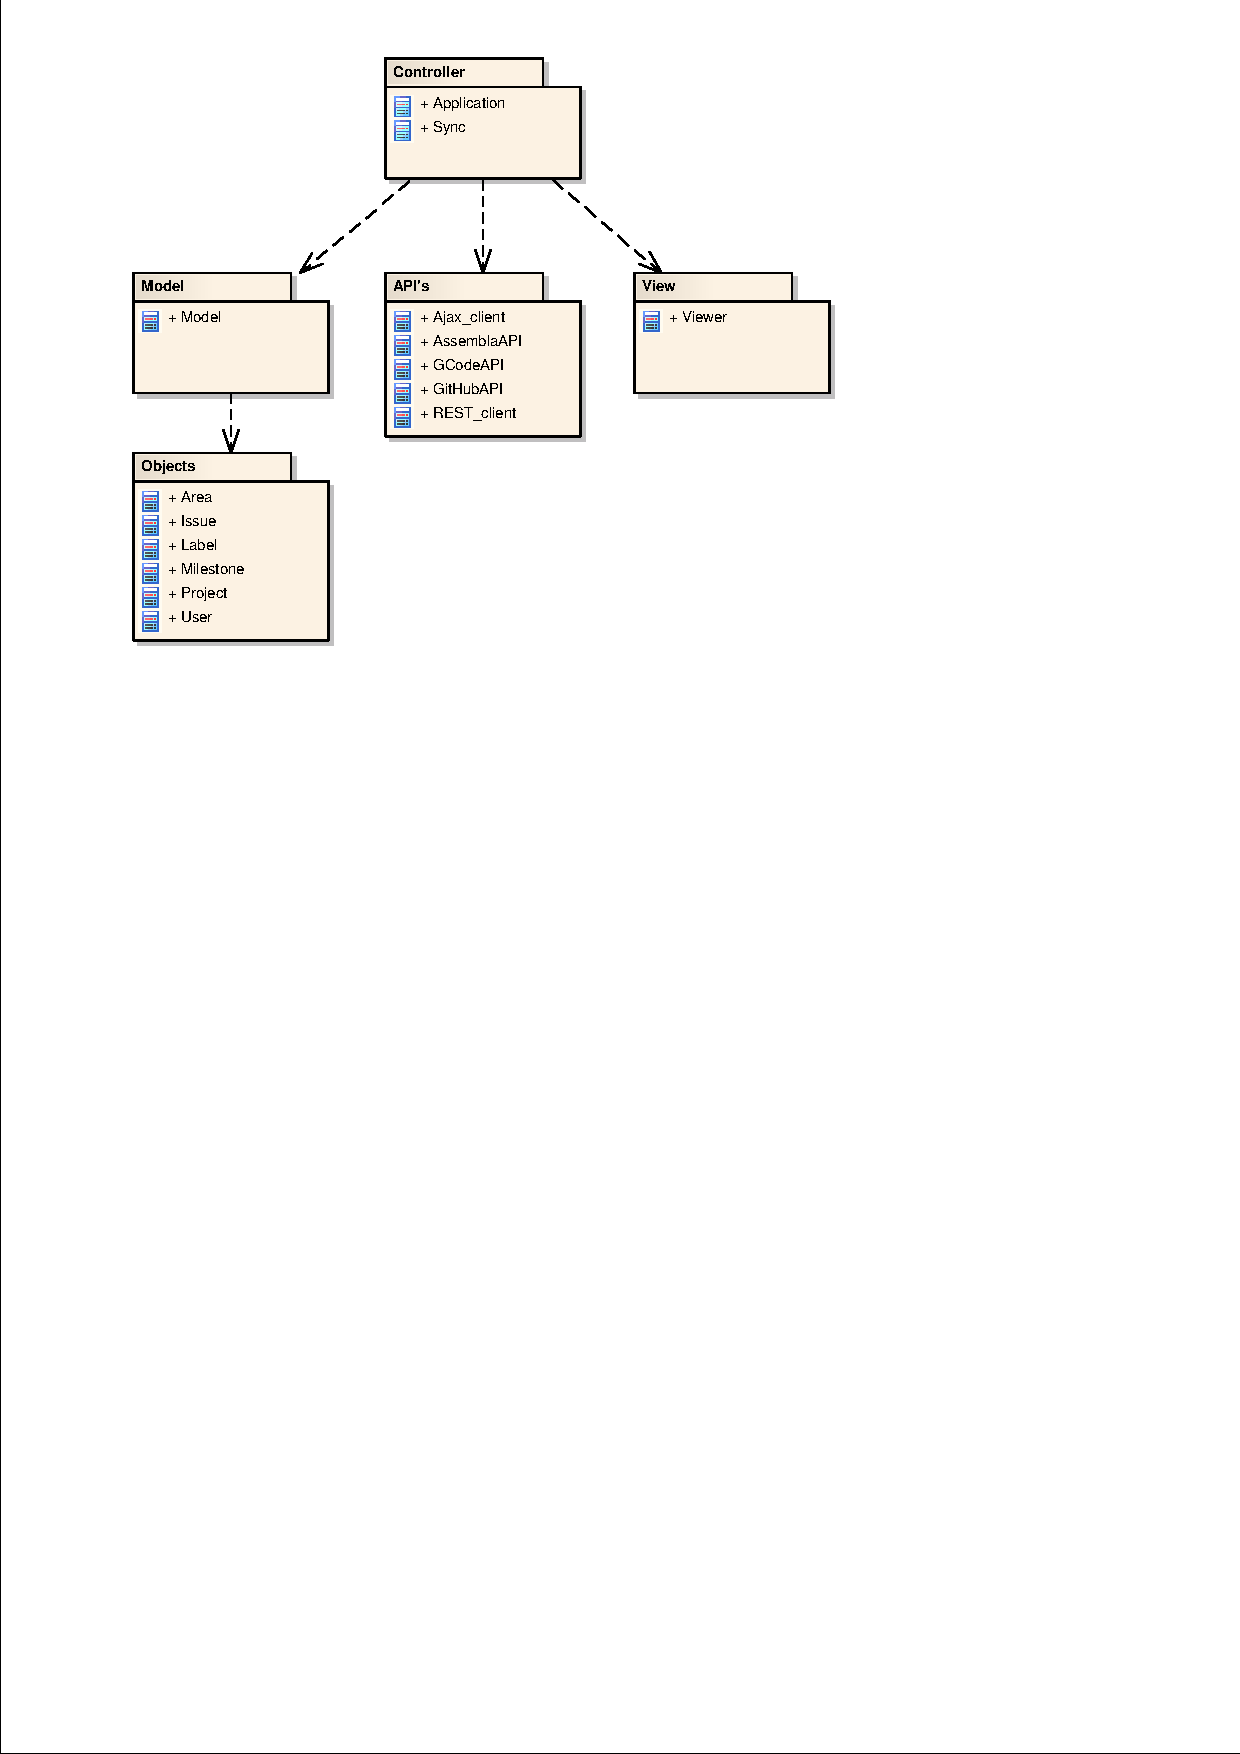
\includegraphics[width=11cm,scale=1,trim=20mm 185mm 60mm 10mm, clip]{figures/class-model}
	\caption{Rozdělení do balíčků}
	\label{fig:class-model}
\end{center}
\end{figure}

\subsection{Controller}

Balíček tříd, které se starají o samotný běh aplikace a synchronizaci se vzdálenými servery.

\subsubsection{Application}

Tato třída je využívána hlavně při startu aplikace. Má dva hlavní úkoly - načíst a naparsovat konfigurační soubor, který je uložený ve formátu JSON, a založit připojení k databázi.

\subsubsection{Sync}

Synchronizace mezi aplikací a vzdálenými servery má na starosti právě tato třída. Přijímá nové objekty z dialogů, předává je do modelové části a stará se o volání odpovídajících API (podle typu projektu). Žádná velká logika v ní není, stará se hlavně o předávání požadavků do jiných vrstev aplikace (model a view).

\subsection{Model}

Balíček tříd, které se starají o komunikaci s databází.

\subsubsection{Model}

V této třídě jsou umístěny všechny metody, které přímo komunikují s databází. Největší skupinou metod jsou ty, které poskytují CRUD (create, read, update, delete) nad všemi entitami zastoupenými v systému. Zároveň je zde několik metod, které usnadňují často používané operace, jako je načítání štítků ke konkrétnímu úkolu nebo zjištění procentuálního dokončení jednotlivých projektů.

\subsection{API's}

Balíček tříd, které jsou používány při komunikaci se vzdálenými servery.

\subsubsection{xxxAPI}

Třídy se sufixem \uv{API} jsou v systému celkem tři (AssemblaAPI, GCodeAPI a GitHubAPI). Každá odpovídá jednomu verzovacímu serveru, se kterým je systém synchronizovatelný. Všechny mají společného předka - abstraktní třídu API - a to z důvodu usnadnění budoucího rozšíření aplikace o další servery. Bohužel v JavaScriptu není implementace dědění úplně dokonalá, takže jde spíš o doporučení než povinnost. Třídy využívají každá svého klienta pro volání vzdálených serverů. U Assembly a Google Code je to REST\_client, GitHub používá Ajax\_client. Zároveň mají na starost naparsování entit do odpovídajícího formátu (JSON nebo XML), aby se dali předat klientovi, který je přepošle ven.

\subsubsection{Ajax\_client}

Tato třída je spolu s tou následující dalším usnadněním budoucího rozšiřování aplikace o spolupráci s dalšími servery. Slouží k odesílání požadavků v podobě AJAXových volání. V momentálním stavu aplikace ji využívá pouze API služby GitHub. Na vstup získává požadavek ve formátu JSON a odesílá ji na stanovenou URL adresu pomocí zvolené metody (POST, PUT, DELETE). Po přijetí odpovědi předá získaný výsledek zpět API do metody, jejíž jméno klient získal při úvodním volání.

\subsubsection{REST\_client}

Protože zbylé dva servery, tzn. Assembla a Google Code, fungují na architektuře označované jako REST (REpresentational State Transfer) bylo nutné vytvořit druhého klienta, který usnadní komunikaci s těmito servery. Požadavky jsou narozdíl od předchozí třídy ve formátu XML souboru. Zpracování odpovědi se příliš neliší od předchozí třídy. Jediný rozdíl tkví v naparsování odpovědi do objektu reprezentujícího XML dokument.

\subsection{View}

Balíček tříd, které mění vizuální stránku aplikace.

\subsubsection{Viewer}

V rámci dodržení architektury MVC došlo k oddělení vytváření vizuální stránky aplikace do samostatné třídy. Ta se stará o výpis seznamu úkolů, projektů a dalších grafických prvků. Grafická stránka aplikace je vytvářena na základě několika šablon, které jsou uloženy v samostatných souborech, aby bylo možné je v budoucnu snadno pozměnit bez ovlivnění funkčnosti aplikace. Takže například výpis úkolů je složen z x částí, kde každá část pochází z jedné šablony, která se opakuje.

\subsection{Entity}

Balíček tříd, které reprezentují jednotlivé entity v systému. Třídy byly již popsány v sekci Metodika - Doménový model.

\section{Bezpečnost}

U webových aplikací je kladen velký důraz na zabezpečení aplikace proti vnějšímu zásahu ať už za účelem získání soukromých informací nebo poškození aplikace. Vytvářená aplikace sice není přímo webová, ale i tak byla otázka zabezpečení důležitá. Nejzranitelnější částí aplikace je samotná komunikace se vzdálenými servery jednotlivých verzovacích systémů. Není totiž možné použít pokročilé zabezpečovací techniky jako je OAuth2 (používá Github) nebo AuthSub proxy (Google Code). V obou případech je totiž nutnou podmínkou fixní URL, na které klientská aplikace běží. Vytvářená aplikace běží přímo na uživatelově počítači a ne někde na vzdáleném serveru a jako taková nemá přidělenou globálně přístupnou URL. Jedinou možností zabezpečení aplikace tak zůstala Basic authentication, u které stačí připojit speciální hlavičku \uv{Authorization} přímo do odesílaného požadavku. Jejím obsahem je slovo \uv{Basic} a zahashované spojení uživatelského jména a hesla kódováním Base64. Tento hash lze snadno přeložit zpět na čitelnou formu, protože účelem toho algoritmu není šifrování přenášených dat ale pouze možnost zapsat binární data do tisknutelných znaků ASCII. Každý z trojice verzovacích systémů (Assembla, Github, Google Code) používá jiný způsob zabezpečení komunikace (tzn. autentizaci a autorizaci). 

\subsection{Zabezpečení serveru Assembla}

U tohoto serveru existuje jediný způsob zabezpečení\cite{assemblaauth} a sice použití Basic Authentication, které vlastně žádné zabezpečení neposkytuje, slouží pouze k autentizaci požadavku na API.

\subsection{Zabezpečení serveru GitHub}

V případě služby Github je situace komplikovanější\cite{github:summary}. Upřednostňovaná forma přihlášení k serveru je OAuth2\cite{github:oauth}, což je protokol sloužící externím aplikacím k požádání o autorizaci bez toho, aby získaly heslo uživatele. Je preferována před Basic Authentication protože umožňuje omezit přístup jen k určitým datům a uživatel může tento přístup kdykoliv zrušit. Postup získání tohoto povolení je jednoduchý. Vývojář nejdřív svou aplikace zaregistruje a tím získá dva údaje: unikátní ID klienta a tajné heslo, které by nemělo být nikde zveřejněno. Pomocí těchto dvou údajů se klientská aplikace autentifikuje u serveru a po vyplnění přihlašovacího jména a hesla je uživatel přesměrován zpět do klientské aplikace s náhodně vygenerovaným tokenem (buď přímo v URL, nebo v hlavičce odpovědi). Tento token je pak používán u každého požadavku na server až do ukončení session. Tento postup je ale pro aplikace běžící na desktopu nepoužitelný protože není kam uživatele přesměrovat. Proto Github zároveň podporuje i Basic Authentication.

\subsection{Zabezpečení serveru Google Code}

Google Code používá službu\cite{googleauth} založenou na podobném principu jako je OAuth2. Zde ale není nutná registrace aplikace přímo na serveru. Aplikace, která vyžaduje přístup k soukromým datům uživatele, a nemůže tedy využit anonymního přístupu, přesměruje uživatele na speciální URL, kde se vyplní uživatelské jméno a heslo a uživatel je posléze přesměrován zpět do klientské aplikace s vygenerovaným AuthSub tokenem uloženým v odpovědi. Obsahem požadavku jsou čtyři údaje:

\begin{enumerate}
\item next - URL, na kterou má být uživatel přesměrován (URL aplikace)
\item scope – určí, že je požadován vstup do Google Code
\item secure – určuje, zda klient požaduje zabezpečený token
\item session – určuje, zda může být token konvertován na multi-use (session) token
\end{enumerate}

Pro aplikace běžící na desktopu je ale nutné použít nižší úroveň zabezpečení – ClientLogin. Ten spočívá v odeslaní požadavku v daném formátu na určitou URL. V odpovědi, pokud je autentizace úspěšná, jsou navrácena tři alfanumerické kódy. Klientskou aplikaci ale zajímá pouze ten poslední, který je použit jako autorizační token při odesílání požadavku (podobně jako se u Basic authentication odesílá Base64 hash). Kamenem úrazu této metody je ale úvodní požadavek, ve kterém je odesláno uživatelské jméno a heslo v čitelné formě přímo v požadavku (konkrétně v POST), takže pokud by provoz na síti někdo odposlouchával, získá snadno přístup do účtu uživatele. Bohužel jiná forma autentizace pro desktopové aplikace neexistuje ani u jedné z těchto tří služeb.

\section{Titanium studio}

\subsection{Představení}

Samotné Titanium Studio je pouze vývojové prostředí, které usnadňuje práci s platformou Titanium. Tato není závislá na operačním systému. Je tak možné vytvářet aplikace zároveň pro Windows, Linux nebo Mac. Stejně tak pokud v budoucnu dojde k vytváření mobilní verzi dané aplikace, je možné některé části kódu znovupoužít a předělat jen grafickou stránku aplikace. Jádrem celé platformy je API\cite{titanium:api}, které je přístupné přes globální objekt Titanium. Přes něj se dají snadno vytvářet další okna aplikace, různá menu a poskytuje snadný přístup k souborům uloženým na filesystému nebo k tabulkám v databázi. Celé API je složené z mnoha modulů, které alespoň ve zkratce představím.

\begin{itemize}
\item Titanium - top-level modul sloužící jako kontejner pro všechny ostatní moduly
\item Titanium.API - přístup do jádra platformy Titanium
\item Titanium.Analytics - správa analytických událostí
\item Titanium.App - správa aktuálně běžící aplikace
\item Titanium.Codec - poskytuje možnost dekódování/zakódování multimédií
\item Titanium.Database - přístup do databáze
\item Titanium.Filesystem - přístup do filesystému
\item Titanium.JSON - umožňuje de/serializovat JSON pole
\item Titanium.Media - správa zvuku
\item Titanium.Network - správa síťových spojení
\item Titanium.Notification - možnost zobrazování notifikací na ploše počítače
\item Titanium.Platform - přístup k funkcím specifické platformy
\item Titanium.Process - možnost vytváření procesů
\item Titanium.UI - správa UI aplikace
\item Titanium.UpdateManager - správa verzování aplikace (instalace updatů)
\item Titanium.Worker - správa vláken Worker
\end{itemize}

\subsubsection{Databáze}

Jako databázový engine se používá SQLite\cite{sqlite}, kde je celá databáze uložena v jednom souboru a tím se snadno zálohuje nebo přenáší na jiný počítač. O připojení k databázi se postará globální objekt, stačí znát jméno databáze, které je možné předem určit. Po připojení se získá objekt, na kterém už lze pokládat dotazy na databázi v jazyce SQL. Jak může takové volání vypadat, ukazuje následující příklad:

\begin{quote}
DB.execute("INSERT INTO images (title, description) VALUES (?, ?)", "test", "description");
\end{quote}

V tomto příkladě je vidět obrana proti útoku SQL Injection, které je realizováno voláním metody s argumenty, které jsou následně escapovány.

\subsubsection{AJAX}

Další velmi důležitou součástí API je mechanismus pro asynchronní volání vzdálených serverů - AJAX. Provádění těchto volání má jednu velkou výhodu oproti tomu samému volání v prohlížeči – není zde problém s cross-domain policy\cite{sameorigin}, což je v zásadě ochrana proti vykonávání JavaScriptu na jiném serveru, kterou mají prohlížeče zabudovánu v sobě. 

Během volání je možné sledovat odpovědi serveru a je možné definovat si funkce, které na tyto události zareagují. API poskytuje plnou kontrolu nad tím jaká data se na server posílají a jaká metoda v rámci protokolu HTTP se použije. API verzovacích serverů totiž rozlišují požadavky i podle této metody. Takže pokud má volání něco na serveru smazat, je třeba použít metodu DELETE. Pokud je naopak účelem něco založit (úkol, projekt, milník), použije se metoda PUT. K běžnému stahování obsahu - čtení - postačí metoda GET příp. POST.

Protože API služeb Assembla a Google Code běží na architektuře REST, je nutné mít možnost posílat voláním i soubory, konkrétně ve formátu XML. Tento požadavek byl poměrně problematický, protože v dokumentaci API není toto dostatečně popsáno. Naštěstí jsou na internetu různé tutoriály, které pomohou a navedou člověka správným směrem. Samotné sestavování AJAXového volání je hodně low-level a člověk musí řešit spousty technických věcí. Například u zmiňovaného posílání souborů je nutné ručně sestavit hlavičku požadavku, aby došel ve správném tvaru na server. Server Assembla například soubor nepřijme, pokud ve volání nepřijde hlavička:

\begin{quote}
Accept : application\slash xml
\end{quote}

\subsubsection{Vytváření oken a nabídek}

Každá aplikace na desktopu sestává z více částí. Hlavní viditelnou částí je samotné okno aplikace. V prostředí Titanium Studia je možné definovat jak toto okno bude velké, zda bude maximalizované a jak s ním bude moct uživatel manipulovat. Všechny tyto volby jsou uloženy v XML souboru, takže se dají snadno upravovat.

Pokud je potřeba za běhu aplikace vytvořit nové okno, umožní to zmiňované API. Nastaví se jeho velikost, poloha, obsah (obvykle HTML soubor) a další volby. Titanium ho pak vykreslí a pak s ním lze dále pracovat. Všechny Javascriptové soubory, které se budou v novém okně používat, jen nutné vložit do toho HTML souboru. A to i když jsou již vloženy do hlavního okna aplikace. Jediné, co se vloží automaticky, je globální objekt Titanium, který zpřístupňuje API.

Většina aplikací na desktopu mívá hlavní menu v šedém pruhu hned na vrchu okna aplikace. I v rámci Titanium Studia je možné toto menu vytvořit. Funguje to jednoduše. Na API stačí zavolat metodu Titanium.UI.createMenu, která vytvoří objekt, reprezentující celé menu. Do něj pak lze buď přidávat další podmenu nebo přímo jednotlivé položky. Menu funguje na principu událostí, takže pokud uživatel na některou z položek klikne, dojde k zavolání metody definované při zakládání dané položky.

\subsection{Výhody a nevýhody}

Mezi hlavní výhody využívání Titanium API rozhodně patří:

\begin{itemize}
\item snadná práce s databází
\item možnost posílat AJAXová volání na vzdálené servery bez omezení
\item snadná práce s UI aplikace (vytváření dalších oken a nabídek)
\end{itemize}

Tyto výhody určitě převyšují dále zmíněné nevýhody, které vyplývají z používání Titanium Studia.

\begin{itemize}
\item debuggování
\item málo chybových hlášení
\end{itemize}

Velkou nevýhodou je rozhodně debugování (nalézání a oprava chyb) aplikace. V rámci běhu aplikace existuje sice možnost sledovat výpis hlášení v okně konzole, ale mnohé chyby se zde neobjeví a aplikace prostě zamrzne. Vývoj se tak občas dost zpomaluje, protože hloupé chyby se hledají obtížně a jeden malý překlep může způsobit velké problémy.

\subsection{Využití API v aplikaci}

Vytvořená aplikace je pevně spojená s Titanium API a nemůže bez něj prakticky existovat. Mezi nejdůležitější využívané funkce patří rozhodně přístup k databázi a filesystému. To jsou funkce, které by byly bez API poměrně obtížně realizovatelné. Je toho ale mnohem víc. Vzhledem k tomu, že jedním z poslání aplikace je synchronizace se vzdálenými servery, je hojně využívána i část síťová, tzn. AJAXová volání. 

Protože JavaScript není úplně objektový jazyk a některé konstrukce nejsou možné, pomohlo Titanium API i zde. Jde například o globální předávání objektů, aby nebylo potřeba je pokaždé vytvářet znovu, což by bylo velké plýtvání prostředky a nejspíš by to výrazně zpomalilo celou aplikaci. Objekty se proto po vytvoření uloží do globální úložiště (ač je to v rozporu s principy objektového programování), které je plně v režii Titanium API a odkud je možné si je kdykoliv vyžádat a vykonávat na nich operace. Takto je například uložené spojení s databází nebo objekt starající se o synchronizaci se vzdálenými servery.

Jak je API v aplikace využíváno, bude nejlépe patrné z nějakého příkladu. Následující model demonstruje workflow přidání nového úkolu do projektu, který je svázán s repozitářem na serveru GitHub. Rámcově lze workflow vyjádřit i textově:

\begin{enumerate}
\item uživatel iniciuje obsluhu události
\item od uživatele se získá nějaký vstup
\item uložení vstupu do databáze
\item zavolání vzdáleného serveru
\item zpracování odpovědi od serveru
\end{enumerate}

\begin{figure}[h]
\begin{center}
	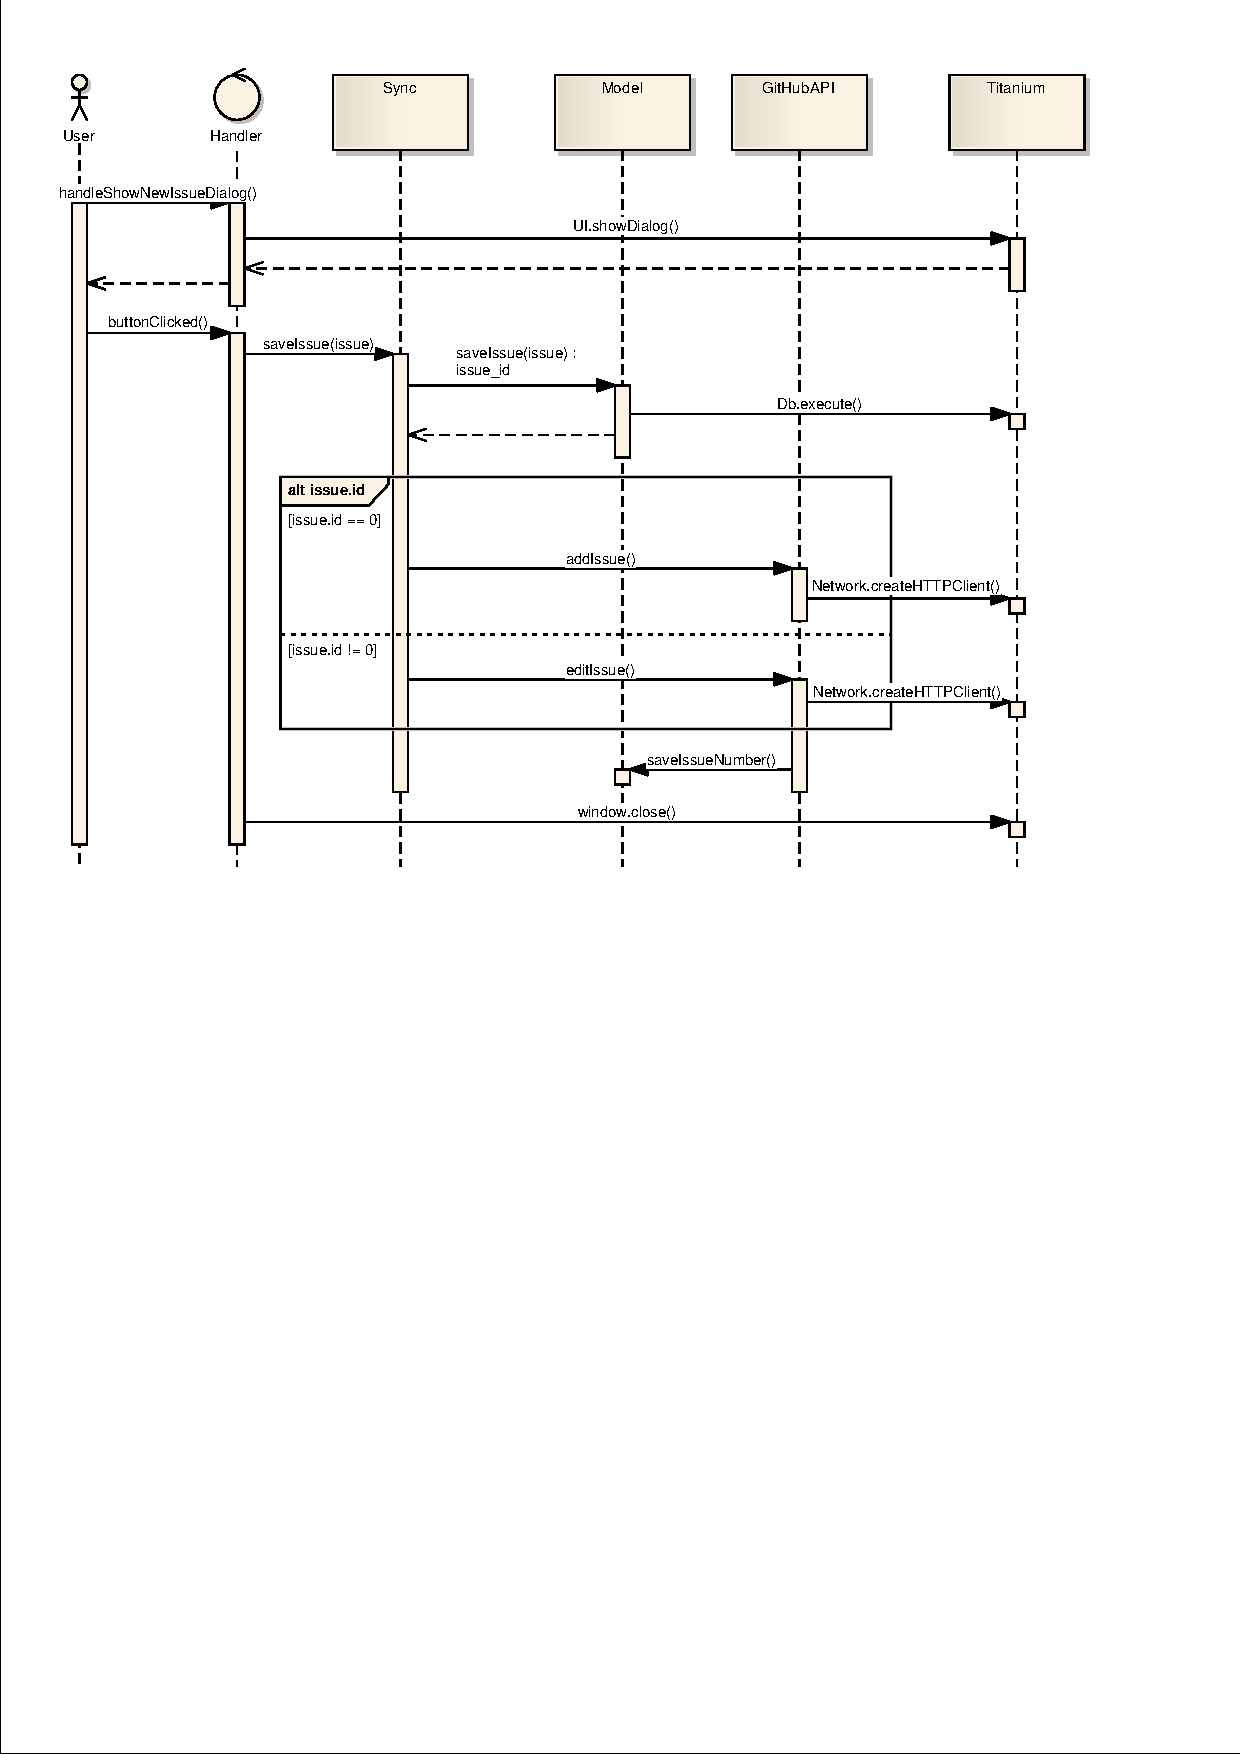
\includegraphics[width=15cm,scale=2,trim=10mm 145mm 10mm 10mm, clip]{figures/vyuziti-api}
	\caption{Využití API v aplikaci}
	\label{fig:vyuziti-api}
\end{center}
\end{figure}

Jak je vidět z diagramu \ref{fig:vyuziti-api}, API je skutečně integrální součástí aplikace a poskytuje spousty důležitých funkcí, které hodně zrychlují a usnadňují vývoj celé aplikace.